%%
%% This is file `sample-sigconf.tex',
%% generated with the docstrip utility.
%%
%% The original source files were:
%%
%% samples.dtx  (with options: `sigconf')
%% 
%% IMPORTANT NOTICE:
%% 
%% For the copyright see the source file.
%% 
%% Any modified versions of this file must be renamed
%% with new filenames distinct from sample-sigconf.tex.
%% 
%% For distribution of the original source see the terms
%% for copying and modification in the file samples.dtx.
%% 
%% This generated file may be distributed as long as the
%% original source files, as listed above, are part of the
%% same distribution. (The sources need not necessarily be
%% in the same archive or directory.)
%%
%% The first command in your LaTeX source must be the \documentclass command.
\documentclass[sigconf]{acmart}
%%%% As of March 2017, [siggraph] is no longer used. Please use sigconf (above) for SIGGRAPH conferences.

%%%% Proceedings format for SIGPLAN conferences 
% \documentclass[sigplan, anonymous, review]{acmart}

%%%% Proceedings format for SIGCHI conferences
% \documentclass[sigchi, review]{acmart}

%%%% To use the SIGCHI extended abstract template, please visit
% https://www.overleaf.com/read/zzzfqvkmrfzn

%%
%% \BibTeX command to typeset BibTeX logo in the docs
\AtBeginDocument{%
  \providecommand\BibTeX{{%
    \normalfont B\kern-0.5em{\scshape i\kern-0.25em b}\kern-0.8em\TeX}}}

%% Rights management information.  This information is sent to you
%% when you complete the rights form.  These commands have SAMPLE
%% values in them; it is your responsibility as an author to replace
%% the commands and values with those provided to you when you
%% complete the rights form.
\setcopyright{acmcopyright}
\copyrightyear{2018}
\acmYear{2018}
\acmDOI{10.1145/1122445.1122456}

%% These commands are for a PROCEEDINGS abstract or paper.
% \acmConference[Woodstock '18]{Woodstock '18: ACM Symposium on Neural
%   Gaze Detection}{June 03--05, 2018}{Woodstock, NY}
% \acmBooktitle{Woodstock '18: ACM Symposium on Neural Gaze Detection,
%   June 03--05, 2018, Woodstock, NY}
% \acmPrice{15.00}
% \acmISBN{978-1-4503-9999-9/18/06}


%%
%% Submission ID.
%% Use this when submitting an article to a sponsored event. You'll
%% receive a unique submission ID from the organizers
%% of the event, and this ID should be used as the parameter to this command.
%%\acmSubmissionID{123-A56-BU3}

%%
%% The majority of ACM publications use numbered citations and
%% references.  The command \citestyle{authoryear} switches to the
%% "author year" style.
%%
%% If you are preparing content for an event
%% sponsored by ACM SIGGRAPH, you must use the "author year" style of
%% citations and references.
%% Uncommenting
%% the next command will enable that style.
%%\citestyle{acmauthoryear}

%%
%% end of the preamble, start of the body of the document source.
\begin{document}

%%
%% The "title" command has an optional parameter,
%% allowing the author to define a "short title" to be used in page headers.
\title{A Study on Kubernetes}

%%
%% The "author" command and its associated commands are used to define
%% the authors and their affiliations.
%% Of note is the shared affiliation of the first two authors, and the
%% "authornote" and "authornotemark" commands
%% used to denote shared contribution to the research.

\author{Udhav Sethi}
\affiliation{\institution{University of Waterloo}}
\email{udhav.sethi@uwaterloo.ca}

\author{Xiyang Feng}
\affiliation{\institution{University of Waterloo}}
\email{x74feng@uwaterloo.ca}

%%
%% By default, the full list of authors will be used in the page
%% headers. Often, this list is too long, and will overlap
%% other information printed in the page headers. This command allows
%% the author to define a more concise list
%% of authors' names for this purpose.
%\renewcommand{\shortauthors}{Trovato and Tobin, et al.}

%%
%% The abstract is a short summary of the work to be presented in the
%% article.
\begin{abstract}
Containerization is taking hold in the datacenter. To leverage the benefits of an isolated environment provided by containers while utilizing resources efficiently, orchestration becomes necessary. Kubernetes is a container orchestration system that allows better tracking, scheduling and operationalizing of containers at scale and eliminates infrastructure complexity. We study and evaluate Kubernetes performance against native application deployment for different workloads. We also conduct a case study on running MongoDB on Kubernetes and discuss the benefits and trade-offs.
\end{abstract}

%%
%% The code below is generated by the tool at http://dl.acm.org/ccs.cfm.
%% Please copy and paste the code instead of the example below.
%%
% \begin{CCSXML}
% <ccs2012>
%  <concept>
%   <concept_id>10010520.10010553.10010562</concept_id>
%   <concept_desc>Computer systems organization~Embedded systems</concept_desc>
%   <concept_significance>500</concept_significance>
%  </concept>
%  <concept>
%   <concept_id>10010520.10010575.10010755</concept_id>
%   <concept_desc>Computer systems organization~Redundancy</concept_desc>
%   <concept_significance>300</concept_significance>
%  </concept>
%  <concept>
%   <concept_id>10010520.10010553.10010554</concept_id>
%   <concept_desc>Computer systems organization~Robotics</concept_desc>
%   <concept_significance>100</concept_significance>
%  </concept>
%  <concept>
%   <concept_id>10003033.10003083.10003095</concept_id>
%   <concept_desc>Networks~Network reliability</concept_desc>
%   <concept_significance>100</concept_significance>
%  </concept>
% </ccs2012>
% \end{CCSXML}

% \ccsdesc[500]{Computer systems organization~Embedded systems}
% \ccsdesc[300]{Computer systems organization~Redundancy}
% \ccsdesc{Computer systems organization~Robotics}
% \ccsdesc[100]{Networks~Network reliability}

%%
%% Keywords. The author(s) should pick words that accurately describe
%% the work being presented. Separate the keywords with commas.
\keywords{Kubernetes, Container, Distributed System}

%% A "teaser" image appears between the author and affiliation
%% information and the body of the document, and typically spans the
%% page.
% \begin{teaserfigure}
%   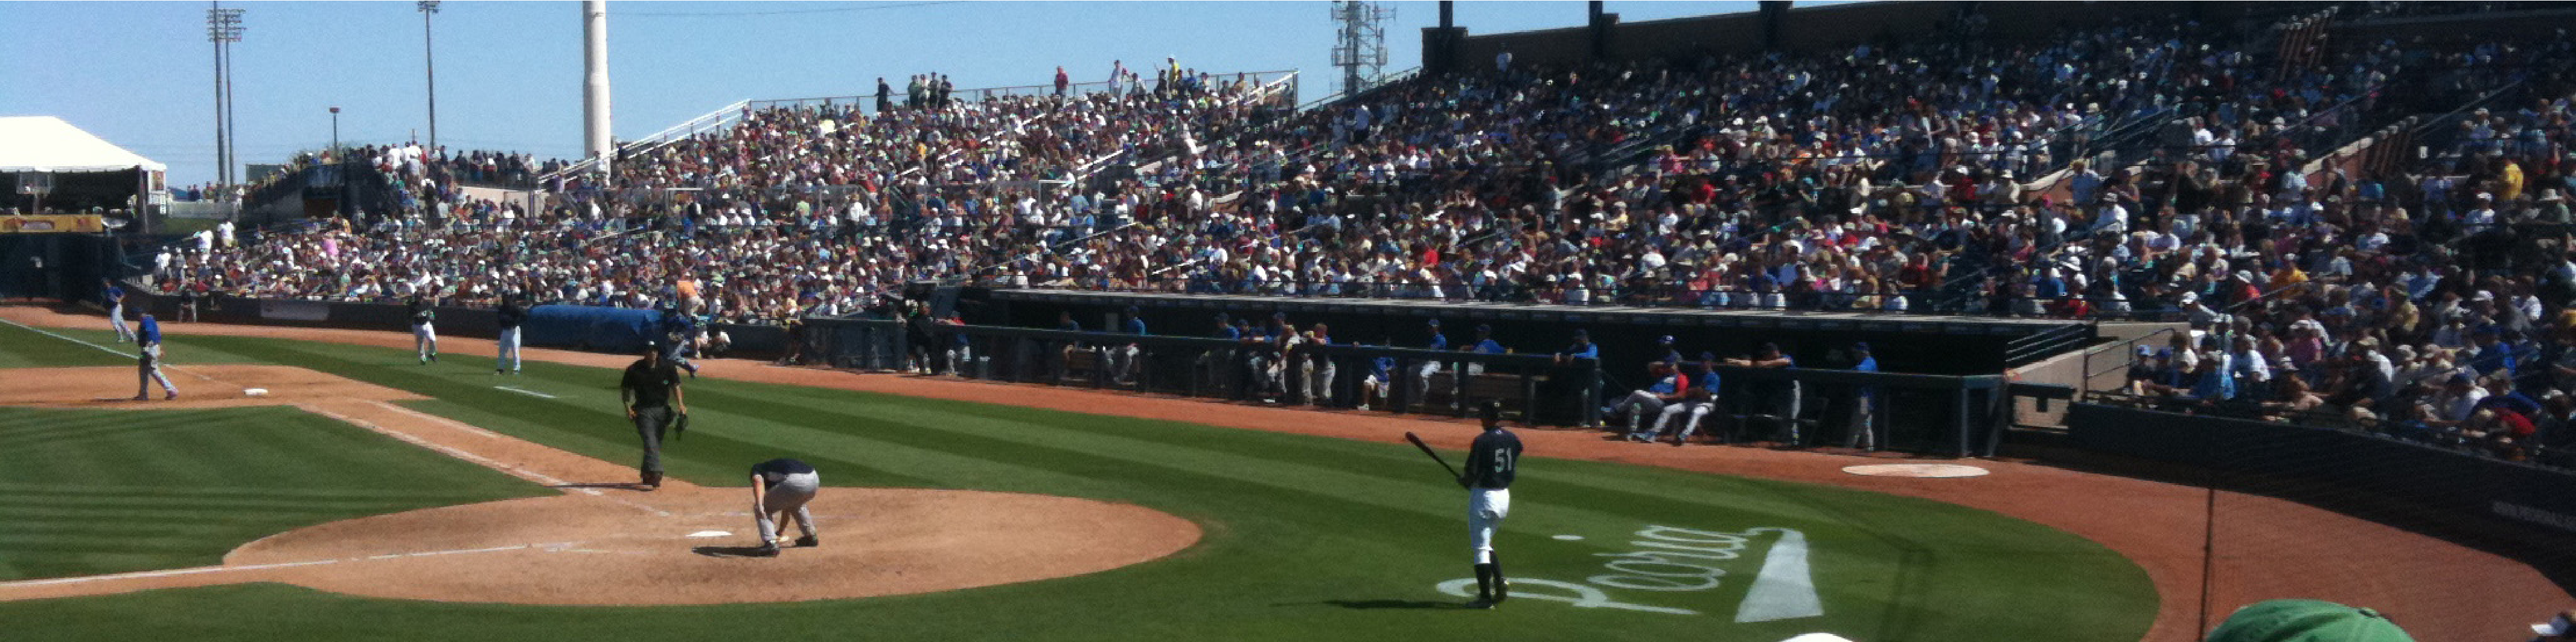
\includegraphics[width=\textwidth]{sampleteaser}
%   \caption{Seattle Mariners at Spring Training, 2010.}
%   \Description{Enjoying the baseball game from the third-base
%   seats. Ichiro Suzuki preparing to bat.}
%   \label{fig:teaser}
% \end{teaserfigure}

%%
%% This command processes the author and affiliation and title
%% information and builds the first part of the formatted document.
\maketitle

\section{Introduction}
In traditional application deployments, applications developed in one computing environment often run into bugs and errors when deployed in another environment. The differences in network topology, storage management, and security policies are some of the variables that lead to issues in the application execution. Containerization attempts to solve this problem by providing an isolated runtime environment to run the application. The application is  bundled together with its dependencies, libraries, binaries, and configuration files into a single package and is run inside a container. Thus, containerization abstracts away the differences in the underlying infrastructure.

Since each container operates independently of others, containers need to be monitored and orchestrated to track all the moving parts and ensure their efficient functioning. Kubernetes is an open-source container-orchestration layer for automating application deployment, scaling, and management. It groups containers that make up an application into logical units for easy management and discovery. Kubernetes enables deployment of a cluster that is highly available, uses resources efficiently, self-heals in case of failures, and scales automatically.

In this paper, we study and evaluate the Kubernetes system. We try to understand its basic functioning, scheduling, and fault-tolerance mechanisms. For evaluation, we first compare the performance of the Kubernetes system in basic tasks, such as ping, CPU intensive and memory intensive workloads against native machine deployments. We then conduct a case study on running the MongoDB application on Kubernetes and investigate the motivation and challenges involved in deployment of such a system. For evaluation, we conduct failover testing on the cluster and also benchmark the performance of the system for the YCSB (Yahoo! Cloud Serving Benchmark) workload.


\section{Basic Concepts}

\subsection{Kubernetes Clusters}
Kubernetes coordinates a cluster of computers running containerized applications and automates the distribution and scheduling of application containers across a cluster in a more efficient way. A Kubernetes cluster consists of a master and workers. The master coordinates all activities in the cluster, such as scheduling applications, maintaining applications' desired state, scaling applications, and rolling out new updates. A worker machine runs the application.

\subsection{Deployments}
A Deployment instructs Kubernetes how to create application instances onto individual Nodes in the cluster.  If the Node hosting an instance goes down or is deleted, the Deployment controller replaces the instance with an instance on another Node in the cluster. This provides a self-healing mechanism to address machine failure or maintenance.

\subsection{Pods}
A Pod is a Kubernetes abstraction for a “logical host” that represents a group of one or more application containers, and some shared resources (such as storage, IP address, ports) for those containers. Containers in a Pod are always co-located and co-scheduled, and run in a shared context on the same Node. A Pod is an atomic unit on the Kubernetes platform.

\subsection{Nodes}
A Node is a worker machine in Kubernetes and may be either a virtual or physical machine. Every Node has a Kubelet, an agent for managing the pods running on the node and communicating with the Kubernetes master, and a container runtime, responsible for pulling the container image from a registry, unpacking the container, and running the application.

\subsection{Services}
A Service is an abstraction which defines a logical set of Pods and enables loose coupling between them. Services enable external traffic exposure, load balancing and service discovery for those Pods. 

\subsection{Scaling}
Horizontal Scaling is accomplished by changing the number of replicas in a Deployment, which creates new Pods are schedules them to Nodes with available resources. Kubernetes also supports autoscaling of Pods, in which the number of pods are automatically scaled up based on observed CPU utilization or other application-provided metrics.

\subsection{Updates}
Kubernetes provides rolling updates, which allows Deployments to be updated with zero downtime by incrementally updating old Pods instances with new ones. If a Deployment is exposed publicly, the Service will load-balance the traffic only to available Pods during the update.

\section{Network}

Modifying the template --- including but not limited to: adjusting
margins, typeface sizes, line spacing, paragraph and list definitions,
and the use of the \verb|\vspace| command to manually adjust the
vertical spacing between elements of your work --- is not allowed.

{\bfseries Your document will be returned to you for revision if
  modifications are discovered.}

\section{Scheduling}

The scheduling framework in Kubernetes attempts to schedule a Pod in two phases, the scheduling cycle and the binding cycle. 

Every Pod that is newly created or unscheduled gets added to a Pod queue. In the scheduling cycle, a pod is dequeued from the queue and the scheduler is responsible for finding the optimal Node for that Pod to run on. Since every Pod and every container in the Pod may have different requirements, it is important to first find the nodes that are capable of running the Pod, and then choosing one of them. The scheduler selects a Node for the Pod in 2 steps: filtering, and scoring. These are described in sections 4.1 and 4.2 below.

\subsection{Filtering Step}
The filtering step finds the set of Nodes where it’s feasible to schedule the Pod. The scheduler follows a defined set of filtering policies to find the list of suitable Nodes. Filtering policies are hard constraints and cannot be violated while finding feasible nodes. Some of these policies are listed below:
\begin{itemize}
\item Matching the hostname specified by the Pod.
\item Checking if the Node meets the resource requirements like CPU and Memory specified by the Pod
\item Checking if the ports requested by a Pod are free on the Node.
\item Matching the Volumes requested by the Pod to the mounted volumes on the Node.
\item Fitering out the Nodes reporting storage/memory/PID pressure.
\item Fitering out nodes with completely full filesystem.
\item Marking a node tainted so that no pods can schedule onto it unless a Pod explicitly tolerates the taint.
\end{itemize}

\subsection{Scoring Step}
Once a list of suitable nodes is determined, the scoring step scores the feasible Nodes and picks a Node with the highest score among the feasible ones to run the Pod. Scoring policies are soft constraints and are followed on a best-effort basis. Some of these policies are a part of the Kubernetes scheduler’s default behavior, while others are user-configurable. Some commonly used policies are listed below:
\begin{itemize}
\item Favouring nodes with fewer/more requested resources.
\item Spreading pods among nodes.
\item Prioritizing nodes according to pod affinity/anti-affinity.
\item Balancing out the resource utilization of nodes.
\item Favouring nodes that already have the container images for that Pod cached locally.
\item Co-locating services that communicate frequently.
\item Simply allocating equal weights to all nodes.
\end{itemize}

On having selected an optimal Node for running a Pod, the binding cycle applies that decision to the cluster. A scheduling or binding cycle can be aborted if the Pod is determined to be unschedulable or if there is an internal error. The Pod will be returned to the queue.

\section{Failure Handling}

\subsection{Replication Controller}
The Replication Controller feature of Kubernetes is responsible for managing the pod lifecycle through supervision of multiple pods across multiple nodes. A Replication Controller ensures that a specified number of pod replicas are up and running at any given time. Depending upon the number of pods specified for the application, the Replication Controller adds more pods or terminates extra pods.

The motivation behind replicating application containers is to achieve reliability, scalability, and load-balancing for the application. The goal of Replication Controller is that the services and their clients should remain oblivious to the underlying process of maintaining a fixed number of replicas in the cluster. The Replication Controller makes it easy to scale the number of replicas up or down, either manually or by an auto-scaling control agent, by simply updating the replicas field.


\subsection{Worker Failure}
The kubelet on each worker node posts a node status to the master every fixed interval of time. The frequency is determined by the node status update frequency (default=40s). If the node is unresponsive for a grace period (default=40s), the node is marked as unhealthy. Once the node is marked unhealthy for longer than the pod eviction grace period (default=5m), all the pods on the node are marked for eviction. Thereafter, no traffic is routed to the pods marked for eviction.

If a node crashes, the above mechanism will kick in and the pods scheduled on the failed node will be evicted from the cluster. In such a scenario, the Replication Controller tries to ensure that the desired number of pods matches its label selector and are operational. It adds the required additional pods to the available healthy nodes in the cluster so that the cluster state is restored.

\subsection{Master Failure}
The master is responsible for managing and coordinating the cluster. If the master goes down, the cluster is no longer able to create new resources, reschedule pods among worker nodes, or respond to worker node failures. Since the other services such as DNS, load balancing etc. continue to function, the application  continues to function normally in the absence of failures. The auto-scaling, self-healing nature of the cluster is no longer operational.

\subsection{Network Partition}
In case of a network partition between the master and a worker node, no traffic is able to be sent to or received from the worker node. In such a scenario, a similar mechanism to worker node failure causes the Replication Controller to perceive those pods to be terminated or deleted. The unreachable node is dropped from the cluster and all its pods are rescheduled to other hosts.


\section{Experiments}
We designed and conducted a set of basic experiments to evaluate the performance of Kubernetes cluster. The application containing these tests was deployed in 3 different environments - a Kubernetes cluster, a Docker container, and bare metal. For each test, we ran the experiment 100 times and recorded the latency values for the average, 10th percentile and 90th percentile case. The experiments are outlined as follows:

\subsection{Ping Test}
In the ping test, a simple "ping" request is sent to the application. The application responds with a simple acknowledgement. This test helps us get an idea of the overall overhead introduced by Kubernetes in the request response path.

\subsection{Memory Intensive Test}
We send a request to the application to perform a memory-intensive task. The request specifies an amount of memory to be allocated and also defines the time interval \texttt{t} for which to define it. The application creates and fills a data structure to occupy the specified size of memory, sleeps for \texttt{t} seconds, and then frees the memory. For our tests, we recorded latencies for requests with memory values of 1GB, 4GB, 8GB, and 16GB. Each size of memory is allocated for \texttt{t=0} seconds, which means the memory is freed right at the end of the time needed to allocate it. 

\subsection{CPU Intensive Test}
For the CPU intensive workload, we compute large exponents of a number. We also specify the number of CPUs we wish to run our computation on. For \texttt{n} number of CPUs, the computation is done \texttt{n} times parallely. We record latencies for requests with 1, 4, 8, and 12 CPUs.

\subsection{results}

\begin{table*}[]
    \centering
    \begin{tabular}{|c|c|c|}
        \hline
        \textbf{Cluster Domain} & \textbf{Service} & \textbf{StatefulSet} \\
        \hline
        cluster.local & default/ngnix & default/web \\
        \hline
        \textbf{StatefulSet Domain} & \textbf{Pod DNS} & \textbf{Pod Hostname} \\
        \hline
        nginx.default.svc.cluster.local & web-\{0..N-1\}.nginx.default.svc.cluster.local & web-\{0..N-1\} \\ 
        \hline
    \end{tabular}
    \caption{Example Network ID}
    \label{tab:Stateful Network}
\end{table*}

\section{Case Study - Running MongoDB on Kubernetes}
MongoDB is a powerful cross-platform NoSQL database application. It is widely used by applications that require flexible data model, scalability and strong performance. Ever since the born of Kubernetes, there has been a line of work on deploying and running MongoDB with Kubernetes done by the open source community. This section will first look into the motivation and challenges of running MongoDB on Kubernetes. It will then cover a detailed deployment process as well as a performance comparison with various workload between native MongoDB cluster and Kubernetes MongoDB cluster.

\subsection{What Kubernetes can offer}
As one of the most widely used orchestration framework, Kubernetes combines the advantages of containers and container scheduling system. Below are some benefits of using containerized applications.
\begin{itemize}
    \item \textbf{Isolation}. In Kubernetes, each container runs application in a completed isolated environment from other containers so that developers do not need to worry about the conflict of configuration between applications. Such isolation also improves the stability of the cluster since the crash of one application cannot affect applications running in a separated container.
    \item \textbf{Automated Deployment}. Kubernetes support elastic scaling of container instances. In case developers want to add, remove containers or do an upgrade on the application, Kubernetes can perform scaling and rolling upgrade automatically without taking down the whole cluster.
    \item \textbf{Automated Rescheduling of Failed Containers}. As described in Section 5, the powerful failure recovery mechanism is arguably the most important reason of running MongoDB on Kubernetes. Consider a native MongoDB cluster with replication set of 3 nodes, in case of node failure, the database administrator has to manually create a new MongoDB instance, configure it with the same setup as other node in the replication set and join it back to the cluster which could be a quite complicated process. However, by using Kubernetes, such node failure can be handled automatically without any admin interference.
\end{itemize}

\subsection{Challenges}
Running MongoDB on Kubernetes is not trivial. This section looks into some of the addition considerations introduced by Kubernetes.
\begin{itemize}
    \item \textbf{Stateful Application}. MongoDB database itself is a stateful application which means a node needs to remember its previous state especially for the data after coming back from failure. However, in contrast, containers are mortal. Everything including storage will disappear when a container goes down. In order to solve this, a persistent volume needs to be attached to MongoDB application containers.  
    \item \textbf{Network Communication}. Nodes within the same MongoDB replication set need to communicate with each other in order to perform back up and synchronization. This implies that every node needs to know each other's network address. However, in a normal Kubernetes service, a pod will be assigned a different ID as well as IP address after coming back from failure which is problematic form communication within the replication set.
    \item \textbf{MongoDB Initialization}. After setting up individual MongoDB instance, developers still need to initialize the MongoDB replication set by executing command inside mongo shell on one the instances. This indicates that developers need to find a way to directly talk with the application running inside the container.
\end{itemize}

\subsection{Kubernetes StatefulSet}
In order to address the challenges mentioned above, Kubernetes introduces a new concept called StatefulSet which is a workload API object used to manage stateful applications. StatefulSet guarantees a stable and unique network together with a stable and persistent storage for the pods running in the cluster.

\subsubsection{Stable Network ID}
Once a pod is created, it will be assigned with a unique integer ordinal within the StatefulSet. The pod then derives its hostname by following the pattern \emph{ \$(statefulset name)-\$(ordinal)}. A StatefulSet also has a Headless Service that controls the domain of its pod. The domain of this service is given in the form of\emph{ \$(service name).\$(namespace).svc.cluster.local}. And each Pod will be assigned a DNS taken the form of \emph{\$(pod name).\$(service domain)}. Table 1 shows an example Stable Network ID for a Kubernetes StatefulSet. 

\subsubsection{Stable Storage}

\subsubsection{Limitations} 
The current implementation of Kubernetes StatefulSet still have the following limitations.
\begin{itemize}
    \item \textbf{Storage Creation} Currently, there are two ways to create persistent storage for a StatefulSet. One is to provision storage through Persistent Volume Provisioner which means in order to enable dynamic storage allocation, developers have to configure the cluster with the Provisioner's service first. The other way is to pre-provision enough static persistent volume and allocate to the MongoDB application running in a StatefulSet which does not scale well. Both methods require enormous time and effort for the administrator to configure.
    \item \textbf{Storage Recollection} Removing a StatefulSet does not delete its associated persistent storage. Kubernetes claims that this is desirable since data safety is more important than resource recollection. However, in the case that developers do not want the associated storage, deletion has to be done manually.
    \item \textbf{StatefulSet Deletion} Deleting a StatefulSet does not guarantee the termination all pods within the StatefulSet. The solution suggested by Kubernetes is to first scale down the StatefulSet to size 0 and then delete. This will make sure all pods terminated prior to deletion.
\end{itemize}

\subsection{Deployment Setup}
We utilize 4 nodes named yellow 12-15 on the SYN cluster, each of which runs a Ubuntu 16.04. All the nodes share 64GB of memory, a 12 core CPU and similary network stack so that they can communicate with each other freely. Two MongoDB replication sets are deployed on yellow 13-15. Yellow 12 is used as the testing server so no application runs on it.

We first deploy a native MongoDB replication set using 3 nodes with yellow 14 as the primary set. All configurations are set to default. User can use MongoDB service by accessing the address \emph{yellow14:27017}. Note that MongoDB does not allow direct writing on secondary replicas so exposing primary replication address is sufficient.

We then deploy an identical MongoDB replication set with Kubernetes. Yellow 13 is used as the Kubernetes master and yellow 14 chosen as the primary replication and exposed its service as type NodePort. For the Kubernetes deployment, we use the StatefulSet approach with dynamic storage allocation as described in the previous section. User can use MongoDB service by accessing \emph{yellow13:\$(exposed service port)}.

\subsection{Failover Test}
A failover test is conducted on Kubernetes MongoDB replication set in order to understand how Kubernetes handles pod failure in a MongoDB replication set. 

The initial state is that 3 pods, each of which has a MongoDB instance, named db-0, db-1 and db-2 are running in the cluster with db-0 being the primary replication. 

\subsection{Benchmark}
\subsubsection{YCSB workload}
\subsubsection{Average Load }
\section{Conclusion}




%%
%% The next two lines define the bibliography style to be used, and
%% the bibliography file.
\bibliographystyle{ACM-Reference-Format}
\bibliography{sample-base}

%%
%% If your work has an appendix, this is the place to put it.
\appendix

\section{Placeholder}


\end{document}
\endinput
%%
%% End of file `sample-sigconf.tex'.
